
\section{\textFlowDesign}

Bei \textFlowDesign{} handelt es sich um eine Methodik, welche dem Entwickler helfen soll
im Voraus saubere Software zu entwerfen. Dabei hilft \textFlowDesign{} etwa bei der
Vermeidung von Abhängigkeiten innerhalb eines Programms durch Entkopplung in einzelne
Module, was ansonsten zu Problemen führen kann.
Datenflüsse werden betrachtet und passende Schnittstellen definiert.

\subsection{System-Umwelt Diagramm}
Beim System-Umwelt Diagramm handelt es sich um eine Betrachtung eines gegebenen oder geplanten Systems, in welcher Interaktionen mit anderen Systemen, Ressourcen und/oder Aktoren dargestellt werden können. Ergänzend hierzu wurde vom Kunden gewünscht, dass bei Interaktionen genauere Details in Listenform hinzugefügt werden können.
Wie im \refLongP{\textMeetingFirst} aufgezeichnet, sollen die einzelnen Interaktionen in der Liste auch mit den passenden Stellen der anderen Diagrammtypen verlinkt sein.


\subsection{Maskenprototyp}
Der Maskenprototyp ist besonders wichtig, um eine grobe Vorstellung zu geben wie das fertig Programm in etwa auszusehen hat. Dieser wird idealerweise in interaktiver Zusammenarbeit, etwa in Kundengesprächen, erstellt. Dabei wurde von unserem Kunden gewünscht, dass bewusst nur rudimentäre Oberflächen erstellbar sind. Damit soll verhindert werden den Eindruck zu vermitteln, dass das Programm bereits fertiggestellt sei.

\subsection{Fluss Diagramm}

Beim Fluss Diagramm wird der Ablauf eines Algorithmus dargestellt. Ein Ablauf kann für sich alleine stehen, oder
anhand des Namens mit einer Aktion eines Maskenprototyp oder als teil eines anderen Algorithmus verknüpft werden.
Ein Flow Diagramm besteht aus Operationen die aneinander gereiht sind, dabei ist das Ergebnis einer Operation der
Parameter für die nächste Operation.
Im folgenden wird auf die Operationen und auf die Notation eingegangen die mit diesem Projekt dargestellt werden kann.
Als Grundlage hat hierbei das ''CheatSheet Flow Design''\cite{flowDesign} gedient. Zuerst werden die einzelnen
Elemente erläutert \refShortP{\textFlowElements} und anschließend die Notation erklärt
\refShortP{\textFlowNotation}.

\subsubsection{\textFlowElements}
\label{\textFlowElements}

Ein Fluss Diagramm hat immer ein Anfang (kleiner Kreis ohne Text) und ein Ende (kleiner Kreis mit X), zwischen dem
die Operationen aufgeführt werden.
\begin{figure}[H]
	\centering
	
\includegraphics[width=\maxwidth{.9\textwidth}]{Element_Start_End.png}
	\caption{Start-Element links, End-Element rechts}
\end{figure}


Eine Operation ist ein größerer Kreis mit dem Namen oder Beschreibung der hier auszuführenden Operation
\begin{figure}[H]
	\centering
	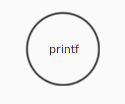
\includegraphics[width=\maxwidth{.9\textwidth}]{Element_Operation.png}
	\caption{Operation-Element}
\end{figure}

Eine Operation kann auch einen Zustand speichern, der über weitere Aufrufe hinweg persistent ist. Dabei wird 
ein Container in die untere rechte Ecke gezeichnet. Dem Zustand kann auch ein Name gegeben werden.
\begin{figure}[H]
	\centering
	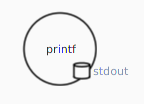
\includegraphics[width=\maxwidth{.9\textwidth}]{Element_Operation_Zustand.png}
	\caption{Operation-Element mit Zustands variable}
\end{figure}

Falls eine Operation auf eine Ressource zugreift, wird dies durch ein Dreieck in der unteren rechten Ecke gezeichnet.
Auch die Ressource kann benannt werden.
\begin{figure}[H]
	\centering
	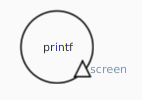
\includegraphics[width=\maxwidth{.9\textwidth}]{Element_Operation_Resource.png}
	\caption{Operation-Element mit Ressourcenzugriff}
\end{figure}

Ein Split-Element stellt die Aufteilung des Programmflusses dar. Das Element wird durch ein Viereck dargestellt
unter dem eine Bezeichnung geschrieben werden kann.
\begin{figure}[H]
	\centering
	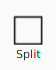
\includegraphics[width=\maxwidth{.9\textwidth}]{Element_Split.png}
	\caption{Split-Element}
\end{figure}

Zum zusammenführen eines Programmflusses wird ein Verbindungselement benötigt. Dies ist ein Strich bei dem
mehrere Flüsse (Abbildung \ref{flowElementVerbindung} links) wieder zu einem zusammengeführt werden (Abbildung
\ref{flowElementVerbindung} rechts).
\begin{figure}[H]
	\centering
	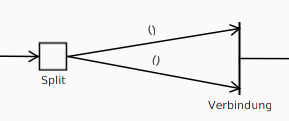
\includegraphics[width=\maxwidth{.9\textwidth}]{Element_Split_Verbindung.png}
	\caption{Verbindungs-Element mit Beispiel}
	\label{flowElementVerbindung}
\end{figure}

Zugriffe auf das Client-System (UI, GUI, WebService, etc \cite{flowDesign}) werden durch ein Portal dargestellt.
Ein Portal ist auch ein Viereck, bei dem sich die Bezeichnung jedoch in dem Viereck befindet. Falls das Fluss Diagramm
von einem Client-System verwendet wird, wird auch das Start und Ende Element durch ein Portal dargestellt.
\begin{figure}[H]
	\centering
	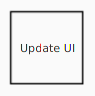
\includegraphics[width=\maxwidth{.9\textwidth}]{Element_Portal.png}
	\caption{Portal-Element}
\end{figure}

Die einzelnen Elemente werden durch Pfeile verbunden auf denen die Übergabedatentypen geschrieben werden. Eine genauere
Erklärung für die Notation kann \refShort{\textFlowNotation} gefunden werden. Optional kann auch an jede beliebige Stelle
eine Kommentarbox eingefügt werden.
\begin{figure}[H]
	\centering
	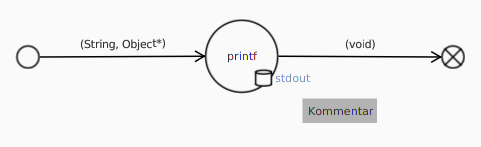
\includegraphics[width=\maxwidth{.9\textwidth}]{Element_connected_comment.png}
	\caption{Beispielhafte Verknüpfung mit Kommentarbox}
\end{figure}

Abhängigkeiten und Schleifen können durch vertikale Verbindungslinien dargestellt werden. Diese Abhängigkeit wird nicht durch einen
Pfeil, sondern durch eine Linie mit einem Punkt am Ende dargestellt; wobei der Punkt bei der Operation ist, von der die andere
abhängig ist.
\begin{figure}[H]
	\centering
	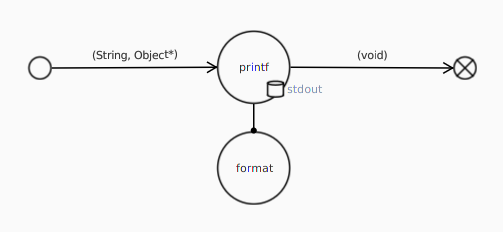
\includegraphics[width=\maxwidth{.9\textwidth}]{Element_connected_dep.png}
	\caption{Beispielhafte Verknüpfung mit Kommentarbox}
\end{figure}

\subsubsection{\textFlowNotation}
\label{\textFlowNotation}